\subsection{非紧区间上函数列极限的积分}

II, p.~52 的定理 1 适用于比规则函数更一般的函数，因为那里只假设这些函数有原函数。特别地可以看出，II, p.~68 的命题 1 仍然适用于如下情形：在区间 I ⊂ R 上，只假设函数 \(f_{\alpha}\) 是分段规则的并且在 I 上有一个积分；然而这个结果以命题 1 的另外两个假设成立为前提，即：1° I 是有界区间；2° \(f_{\alpha}\) 在 I 上一致收敛于 f。当这些条件之一不再满足时，II, p.~68 的公式 (1) 可能失效：可能这两项之一不存在，也可能两项都存在但取不同的值。

例如，若 \(f_{n}\) 是 {]}0, 1{]} 上的规则函数，由 \(f_{n}(x) = n\)（当 \(0 < x < 1 / n\)）与 \(f_{n}(x) = 0\)（当 \(1 / n \leqslant x \leqslant 1\)）定义，则序列 \((f_{n})\) 在含于 \([0, 1]\) 的每个紧区间上一致收敛于 0，但在 \([0, 1]\) 上不一致收敛，且对每个 n 有 \(\int_{0}^{1} f_{n}(t) dt = 1\)。有一个 \(\int_{0}^{1} f_{n}(t) dt\) 不趋于任何极限的例子：把前面的序列 \((f_{n})\) 换成序列 \(((-1)^{n} f_{n})\)，后者同样在含于 \([0, 1]\) 的每个紧区间上一致收敛于 0。

另一方面，在无界区间 I = {[}0, +∞{[} 上，设 \(f_{n}\) 是这样的规则函数：\(f_{n}(x) = 1/n\)（当 \(n^{2} \leqslant x \leqslant (n+1)^{2}\)），而当 x 在 I 中取其他值时 \(f_{n}(x) = 0\)（\(n \geqslant 1\)）；序列 \((f_{n})\) 在 I 上一致收敛于 0，但积分 \(\int_{0}^{+\infty} f_{n}(t) dt = (2n+1)/n\) 当 n 无限增大时趋于 2。

\pandocbounded{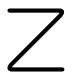
\includegraphics[keepaspectratio]{images/part001_bd86b8f3.jpg}}

换言之，当 I 无界时，若以 \(\mathcal{I}\) 表示由 I 上的规则函数 \(\mathbf{f}\)（取值于 E 且在 I 上有一个积分）所构成的向量空间，则映射 \(\mathbf{f} \mapsto \int_{\mathrm{I}} \mathbf{f}(t) dt\) 在 \(\mathcal{I}\) 赋以 I 上一致收敛的拓扑之后不是连续的（参见 II, p.~53, 推论 2）。

我们将在下列假设之下寻求保证命题 1 成立的充分条件：

\(1^{\circ}\) I 是 \(\mathbf{R}\) 中的任意区间，函数 \(\mathbf{f}_{\alpha}\) 在 I 上是规则的，并且在 I 上有一个积分；

\(2^{\circ}\) 族 \((\mathbf{f}_{\alpha})\) 在含于 I 的每个紧区间上一致收敛于 \(\mathbf{f}\)（关于滤子 \(\mathfrak{F}\)）。

以 \(\mathfrak{K}(\mathrm{I})\) 表示含于 I 的紧区间所成的有向集（II, p.~64），II, p.~68 的公式 (1) 的左端可以写成 \(\lim_{\mathfrak{F}}\left(\lim_{\mathrm{J}\in \mathfrak{K}(\mathrm{I})}\int_{\mathrm{J}}\mathbf{f}_{\alpha}(t)dt\right)\)；
另一方面，考虑到命题 1（II, p.~68）以及族 \((\mathbf{f}_{\alpha})\) 在每个紧区间 \(J \subset I\) 上一致收敛这一事实，(1)（II, p.~68）的右端可以写成 \(\lim_{\mathrm{J} \in \mathfrak{K}(\mathrm{I})} \left( \lim_{\mathfrak{F}} \int_{\mathrm{J}} \mathbf{f}_{\alpha}(t) dt \right)\)。由此看出，只要
对映射 (J, \(\alpha\) ) \(\mapsto \int_{J} f_{\alpha}(t) dt\) 关于滤子 F 以及关于有向集 K(I) 的截口滤子 \(\Phi\) 可以交换极限，II, p.~19 的命题 1 就可以推广。现在，我们知道使这一交换合法的一个充分条件，即映射 (J, \(\alpha\) ) \(\mapsto \int_{J} f_{\alpha}(t) dt\) 关于乘积滤子 \(\Phi \times F\) 的极限存在（Gen.~Top., I, p.~81, 定理 1 的推论）。我们将把这个条件变换为一个等价的、更便于使用的条件。

首先，由于 E 是完备的，为使 \((\mathbf{J}, \alpha) \mapsto \int_{\mathbf{J}} \mathbf{f}_{\alpha}(t) dt\) 关于 \(\Phi \times F\) 有极限，必须且只需：对每个 \(\varepsilon > 0\)，存在一个紧区间 \(J_{0} \subset I\) 和一个集 \(M \in F\)，使得对 M 中任意的元素 \(\alpha\)、\(\beta\) 以及任意的含于 I 的紧区间 \(J \supset J_{0}\)，有

\[
\left\| \int_ {J _ {0}} \mathbf {f} _ {\alpha} (t) d t - \int_ {J} \mathbf {f} _ {\beta} (t) d t \right\| \leqslant \varepsilon .\tag{4}
\]

另一方面我们将证明，这个条件本身等价于下列条件：对每个 \(\varepsilon > 0\)，存在一个紧区间 \(J_0 \subset I\) 和一个集 \(M \in \mathfrak{F}\)，使得对任意的 \(\alpha\)（属于 \(M\)）以及任意的紧区间 \(J \supset J_0\)（含于 \(I\)），有

\[
\left\| \int_ {J _ {0}} \mathbf {f} _ {\alpha} (t) d t - \int_ {J} \mathbf {f} _ {\alpha} (t) d t \right\| \leqslant \varepsilon .\tag{5}
\]

的确，明显可见后一条件是必要的；反之，若它满足，则（由 \((\mathbf{f}_{\alpha})\) 在每个紧区间上的一致收敛性）存在一个集 \(N \in F\)，使得对 N 中任意的 \(\alpha\)、\(\beta\)，有

\[
\left\| \int_ {\mathrm{J} _ {0}} \mathbf {f} _ {\alpha} (t) d t - \int_ {\mathrm{J} _ {0}} \mathbf {f} _ {\beta} (t) d t \right\| \leqslant \varepsilon ;\tag{6}
\]

因而有 \(\left\|\int_{J_{0}}\mathbf{f}_{\alpha}(t)dt-\int_{J}\mathbf{f}_{\beta}(t)dt\right\|\leqslant2\varepsilon\)（对任意的 \(\alpha\) 与 \(\beta\)（属于 \(M\cap N\in\mathfrak{F}\)）以及任意的紧区间 \(J\supset J_{0}\)）。

最后，II, p.~65 的引理使我们能把后一条件写成下列等价形式：对每个 \(\varepsilon > 0\)，存在一个紧区间 \(\mathbf{J}_0 \subset \mathbf{I}\) 和一个集 \(\mathbf{M} \in \mathfrak{F}\)（依赖于 \(\varepsilon\)），使得对每个紧区间 \(\mathbf{K} \subset \mathbf{I}\)（与 \(\mathbf{J}_0\) 无公共内点）以及每个 \(\alpha \in \mathbf{M}\)，有 \(\left\| \int_{\mathbf{K}} \mathbf{f}_{\alpha}(t) dt \right\| \leqslant \varepsilon\)。

最常用的，是一个更强的条件，它是在上述结论中假设集 M 不依赖于 \(\varepsilon\) 而得到的：

定义 1. 我们说积分 \(\int_{\mathrm{I}} \mathbf{f}_{\alpha}(t) dt\) 对 \(\alpha \in \mathrm{A}\) 一致收敛（或在 \(\mathrm{A}\) 上一致收敛），如果对每个 \(\varepsilon > 0\)，存在一个紧区间 \(\mathrm{J}_0 \subset J\)，使得对每个紧区间 \(\mathrm{K} \subset \mathrm{I}\)（与 \(\mathrm{J}_0\) 无公共内点）以及每个 \(\alpha \in \mathrm{A}\)，有

\[
\left\| \int_ {K} \mathbf {f} _ {\alpha} (t) d t \right\| \leqslant \varepsilon .\tag{7}
\]

这个定义等价于说：映射族 \(\alpha\mapsto\int_{J}\mathbf{f}_{\alpha}(t)dt\) 在 A 上一致收敛（收敛于映射 \(\alpha\mapsto\int_{I}\mathbf{f}_{\alpha}(t)dt\)），即关于滤子 \(\Phi\)（\(\Re(I)\) 的截口滤子）而言；诸积分 \(\int_{I}\mathbf{f}_{\alpha}(t)dt\) 中的每一个更是收敛的（反之不真）；此外，由我们刚才所见（或由 Gen.~Top., X, p.~281, 推论 2）：

命题 3. 设 \((\mathbf{f}_{\alpha})\) 是区间 I 上的一个规则函数族，满足：\(1^{\circ}\) 关于滤子 \(\mathfrak{F}\)，族 \((\mathbf{f}_{\alpha})\) 在含于 I 的每个紧区间上一致收敛于一个函数 \(\mathbf{f}\)（在 I 上是规则的）；\(2^{\circ}\) 积分 \(\int_{I} \mathbf{f}_{\alpha}(t) dt\) 对每个 \(\alpha \in A\) 一致收敛。在这些假设之下，积分 \(\int_{I} \mathbf{f}(t) dt\) 收敛，且有

\[
\lim _ {\mathfrak {F}} \int_ {\mathrm{I}} \mathbf {f} _ {\alpha} (t) d t = \int_ {\mathrm{I}} \mathbf {f} (t) d t.\tag{8}
\]

例如当 I 是有界区间、\(\mathbf{f}_{\alpha}\) 在 I 上一致有界且在含于 I 的每个紧区间上一致收敛于 \(\mathbf{f}\) 时，命题 3 的假设满足；事实上，若 \(\| \mathbf{f}_{\alpha}(x)\| \leqslant h\) 对一切 \(x\in \mathrm{I}\) 与一切 \(\alpha\) 成立，且 \(\mathrm{J}_0\) 使得 I 与 \(\mathrm{J}_0\) 的长度之差 \(\leqslant \varepsilon /h\)，则对每个区间 \(\mathrm{K}\subset \mathrm{I}\)（与 \(\mathrm{J}_0\) 无公共内点），条件 (7) 满足。

与 II, p.~68 的命题 1 一样，命题 3 的两个推论在应用中很重要：

推论 1. 设 \((\mathbf{f}_{n})\) 是任意区间 I 上的一个规则函数序列，在含于 I 的每个紧区间上一致收敛于函数 f；若积分 \(\int_{I} \mathbf{f}_{n}(t) dt\) 一致收敛，则积分 \(\int_{I} \mathbf{f}(t) dt\) 收敛，且

\[
\lim _ {n \to \infty} \int_ {\mathrm{I}} \mathbf {f} _ {n} (t) d t = \int_ {\mathrm{I}} \mathbf {f} (t) d t.\tag{9}
\]

注记。这个推论中所加的假设对公式 (9) 的成立是充分的，但不是必要的；以后我们将在推广积分概念的同时推广这个公式（见 INT, IV），并得到弱得多的条件。

推论 2. 设 A 是拓扑空间 F 的一个子集，f 是 I × A 到 R 上的完备赋范空间 E 中的一个映射，使得对每个 \(\alpha \in A\)，函数 \(x \mapsto \mathbf{f}(x, \alpha)\) 在 I 上是规则的。若一方面，函数 \(x \mapsto \mathbf{f}(x, \alpha)\) 在含于 I 的每个紧区间上一致收敛于函数 \(x \mapsto \mathbf{f}(x)\)（当 \(\alpha\) 趋于 \(\alpha_{0} \in \overline{A}\) 而保持属于 A 时）；若另一方面，积分 \(\int_{I} \mathbf{f}(x, \alpha) dx\) 在 A 上一致收敛，则积分 \(\int_{I} \mathbf{f}(x) dx\) 收敛，且有

\[
\lim _ {\alpha \rightarrow \alpha_ {0}, \alpha \in A} \int_ {I} \mathbf {f} (x, \alpha) d x = \int_ {I} \mathbf {f} (x) d x.\tag{10}
\]

特别地：

命题 4（“反常积分对参数的连续性”）。设 F 是紧空间，I 是 R 中的任意区间，f 是 I × F 到 R 上的完备赋范空间 E 中的连续映射；若积分 \(\mathbf{h}(\alpha) = \int_{\mathrm{I}} \mathbf{f}(x, \alpha) dx\) 在 F 上一致收敛，则它是 \(\alpha\) 在 F 上的连续函数。

由于 II, p.~69 的命题 2，本命题也可由连续函数的一致极限的连续性（Gen.~Top., X, p.~282, 定理 2）得出。

